% !TEX TS-program = xelatex

\chapter{Symbolic modeling with Julia Plasm}
\label{chapt:5}

Symbolic modeling is a semantic approach to knowledge representation and processing. A  symbolic approach to design with the aim of representing information and computation uses names to define the meaning of represented knowledge explicitly. The geometric knowledge is described here by Julia's names, which are chosen suitably for functionals, functions, formal and actual parameters, and finally for objects, fields, classes, attributes, methods, relations, etc. In this chapter, we give many examples of high-level Plasm programming, from topological, linear, and affine operators, to geometric mapping of complexes and grids to generate linearized approximation of curved manifold of intrinsic dimensions 1, 2, and 3. i.e., depending on such number of parameters; say, curves, surfaces, thin, and bulk solids.



\section{ Primitive generators}\label{sect:5-1}

Here, we introduce both single objects and aggregates of cells, typically by grid and mesh generators, resulting in a single |Hpc| value after the evaluation.


\subsection*{Higher order and partial functions}\label{sect:5-1-0}

As we have already seen in Section \ref{}, Julia |Plasm| is higher-level since allows for function that take functions as argument and/or may return a function value.  All functions are objects of Julia |Function| type. As objects (holding a reference to the function code), can be assigned to a name (identifier).

\begin{definition}[Function order] The \emph{order} of an object of |Function| type is the number of applications to actual parameters needed to return the ultimate actual value,  not a partial function value (needing further parameters).
\end{definition}

\begin{coding}[\sf  INTERVALS(size::Numrber)(n::Int)] In this example we show a second-order function (requiring two applications) that generates a 1D complex made by |n| line segments of total given |size| length.
\begin{lstlisting}[language=JuliaLocal, style=julia, mathescape=true]
segments = INTERVALS(10::Number)(4::Int)		#=
Hpc(MatrixNd(2), Geometry([[0.0], [2.5], [5.0], [7.5], [10.0]], hulls=[[1, 2], [2, 3], [3, 4], [4, 5]]))		=#
\end{lstlisting}
Note that |segments| value is 1D since its 11 vertices have one coordinate. 
\end{coding}


\begin{coding}[\sf  QUOTE(measures::Array{Number})]\
The formal parameter is an array of signed numbers.
\begin{lstlisting}[language=JuliaLocal, style=julia, mathescape=true]
two_aligned_segments = QUOTE([1,-2.5,1])			#=
Hpc(MatrixNd(2), Geometry([[0.0], [1.0], [3.5], [4.5]], hulls=[[1, 2], [3, 4]]))	=#
\end{lstlisting}
Positive numbers denote solid intervals of a given size; negative numbers denote hollow space, i.e., displacement of following segments. Successive negative numbers are allowed.\end{coding}


\begin{coding}[\sf  Q(measure::Number)]\
The formal parameter is a signed number. 
\begin{lstlisting}[language=JuliaLocal, style=julia, mathescape=true]
segment = Q(10)
Hpc(MatrixNd(2), Geometry([[0.0], [10.0]], hulls=[[1, 2]]))
\end{lstlisting}
A single |segment| of given size.
\end{coding}


\subsection*{Single convex cell}\label{sect:5-1-1}

Julia |Plasm| contains a great library of generator functions of very simple objects made by a single convex cell, and completely specified by its set of vertices only. 
Few examples follow; Other examples can be extracted or generated by the user looking at file |src/fenvs.jl|, including the Platonic solids. The multidimensional $d$-permutaheron is generated in Coding \ref{4-2-permutahedron}. 

\begin{coding}[\sf  CUBOID(size)]\
Multidimensional cuboid with |sizes::Vector{Number}|.
\begin{lstlisting}[language=JuliaLocal, style=julia, mathescape=true]
CUBOID([1])			#=
Hpc(MatrixNd(2), Hpc(MatrixNd(2), Geometry([[0.0], [1.0]], hulls=[[1, 2]]))) =#

CUBOID([1,2])			#=
Hpc(MatrixNd([[1.0, 0.0, 0.0], [0.0, 1.0, 0.0], [0.0, 0.0, 2.0]]), Hpc(MatrixNd(3), Geometry([[0.0, 0.0], [1.0, 0.0], [1.0, 1.0], [0.0, 1.0]], hulls=[[1, 2, 3, 4]]))) =#

CUBOID([1,2,3])			#=
Hpc(MatrixNd([[1.0, 0.0, 0.0, 0.0], [0.0, 1.0, 0.0, 0.0], [0.0, 0.0, 2.0, 0.0], [0.0, 0.0, 0.0, 3.0]]), Hpc(MatrixNd(4), Geometry([[0.0, 0.0, 0.0], [1.0, 0.0, 0.0], [0.0, 1.0, 0.0], [1.0, 1.0, 0.0], [0.0, 0.0, 1.0], [1.0, 0.0, 1.0], [0.0, 1.0, 1.0], [1.0, 1.0, 1.0]], hulls=[[1, 2, 3, 4, 5, 6, 7, 8]]))) =#

CUBOID([1,2,3,4])			#=
Hpc(MatrixNd([[1.0, 0.0, 0.0, 0.0, 0.0], [0.0, 1.0, 0.0, 0.0, 0.0], [0.0, 0.0, 2.0, 0.0, 0.0], [0.0, 0.0, 0.0, 3.0, 0.0], [0.0, 0.0, 0.0, 0.0, 4.0]]), Hpc(MatrixNd(5), Geometry([[0.0, 0.0, 0.0, 0.0], [1.0, 0.0, 0.0, 0.0], [0.0, 1.0, 0.0, 0.0], [1.0, 1.0, 0.0, 0.0], [0.0, 0.0, 1.0, 0.0], [1.0, 0.0, 1.0, 0.0], [0.0, 1.0, 1.0, 0.0], [1.0, 1.0, 1.0, 0.0], [0.0, 0.0, 0.0, 1.0], [1.0, 0.0, 0.0, 1.0], [0.0, 1.0, 0.0, 1.0], [1.0, 1.0, 0.0, 1.0], [0.0, 0.0, 1.0, 1.0], [1.0, 0.0, 1.0, 1.0], [0.0, 1.0, 1.0, 1.0], [1.0, 1.0, 1.0, 1.0]], hulls=[[1, 2, 3, 4, 5, 6, 7, 8, 9, 10, 11, 12, 13, 14, 15, 16]]))) =#
\end{lstlisting}
Cuboids of given sizes. Of course, the unit hypercube in $\E^6$ has |size = [1,1,1,1,1,1]|. 
\end{coding}

The |Plasm| coding of the “icosphere”, polyhedral approximation of the 2-sphere obtained by subdividing the |ICOSAHEDRON()| surface is given here, starting from the Platonic solid. The generation method is extremely simple. We obtain the vertices at step $i+1$ by adding to the vertices at step $i$ those obtained by subdivision of all edges. Ma make use of theHpc structure and the Lar structure.


\begin{coding}[\sf  ICOSPHERE(seed::Hpc)::Hpc]\
First we generate the cell complex of the input |obj| using the |LAR| combinator, then for each edge we compute the mean point, then we aggregate to the old vertices the new ones, scaled by the factor |r1/s1| built with the distance from |[0,0,0]| center of both models.
\begin{lstlisting}[language=JuliaLocal, style=julia, mathescape=true]
function ICOSPHERE(obj::Hpc)::Hpc
   W  = LAR(obj).V
   EV = LAR(obj).C[:EV]
   W  = [W[:,k] for k=1:size(W,2)]
   V  = [(W[v1]+W[v2])./2 for (v1,v2) in EV]
   r1 = sqrt(sum(W[1].^2))
   s1 = sqrt(sum(V[1].^2))
   CONVEXHULL([W; V*(r1/s1)]);
end
\end{lstlisting}
Finally, the |[W; V*(r1/s1)]::Vector{Vector{Float64}}| made by old vertices and by new scaled ones is given to the operator |CONVEXHULL| that transforms such a |Vector| of point (|Vector{Float64}|) in their geometric \emph{convex hull}.
Just remember that such polyhedra are convex sets, hence they have a \emph{single} (convex) cell. \begin{lstlisting}[language=JuliaLocal, style=julia, mathescape=true]
out0 = ICOSAHEDRON();   VIEW(out0)
out1 = ICOSPHERE(out0); VIEW(out1)
out2 = ICOSPHERE(out1); VIEW(out2)
out3 = ICOSPHERE(out2); VIEW(out3)
...		
\end{lstlisting}
Successive approximations of icosphere with 12, 42, 162, 600, etc., vertices.
Let’s remark the extreme simplicity of such polyhedral generations.
\end{coding}

\begin{figure}[htbp] %  figure placement: here, top, bottom, or page
   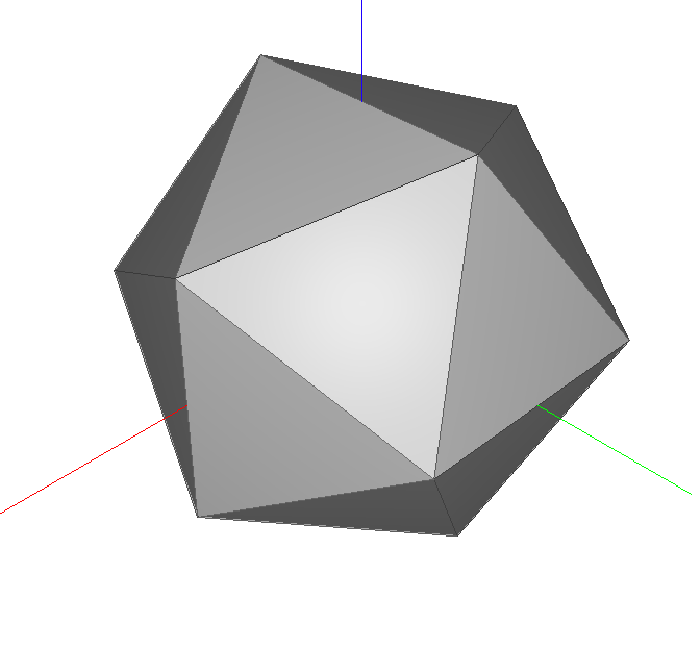
\includegraphics[width=0.34\linewidth]{chapter-05/figs/icosphere0}%
   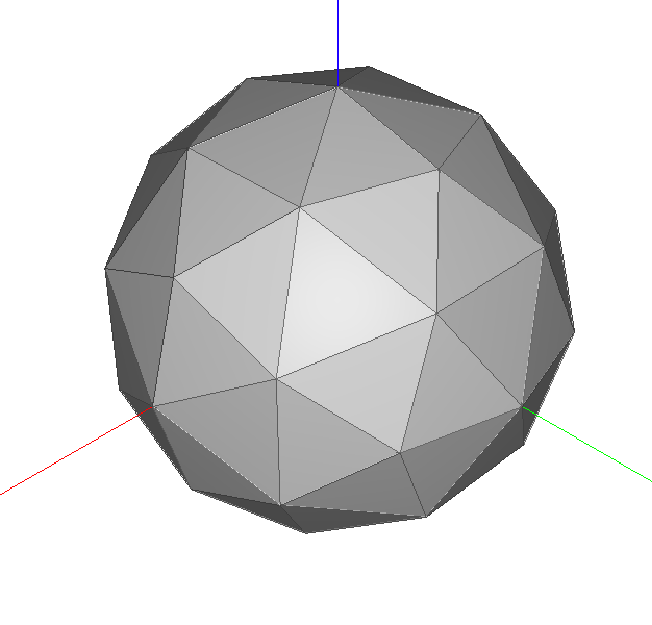
\includegraphics[width=0.33\linewidth]{chapter-05/figs/icosphere1}%
   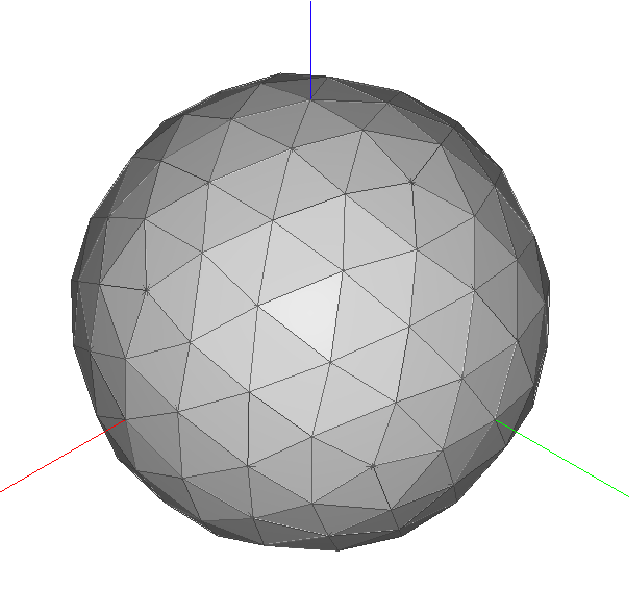
\includegraphics[width=0.325\linewidth]{chapter-05/figs/icosphere2}%
\hfill
\caption{(a) Icosahedron; (b) icosphere with 42 vertices; (c)  icosphere with 162 vertices. }
\label{5:icospheres}
\end{figure}



\subsection*{Multiple cell objects}\label{sect:5-1-1}


The functions |INTERVALS| or |QUOTE| may be used to create many types and patterns of grid geometries.

\begin{script}[Building frame]\
First we give the main dataset of a building frame, by “quoting” the side measures of 2D design plan:
\begin{lstlisting}[language=JuliaLocal, style=julia, mathescape=true]
# Longitudinal trusses
Y = QUOTE([0.3, -6, 0.3, -6, 0.3])
# transverse beams
X = QUOTE([0.3, -3, 0.3, -4.2, 0.3, -3, 0.3])
# vertical measurements
Z = QUOTE([3,0.3])
\end{lstlisting}
Then, an alternate set of |INTERVALS| vector parameters are generated by Julia broadcast |.*| of the scalar |-1|, in order to invert all the signs.
\begin{lstlisting}[language=JuliaLocal, style=julia, mathescape=true]
X1 = QUOTE([0.3, -3, 0.3, -4.2, 0.3, -3, 0.3].* -1)
Y1 = QUOTE([0.3, -6, 0.3, -6, 0.3].*-1)
Z1 = QUOTE([3,-0.3].*-1)
\end{lstlisting}
Below, the 3D |frame| subsystems are generated. They are the $C_3$ basis of a local cellular complex. Note the variation pattern at |trusses1|.
\begin{lstlisting}[language=JuliaLocal, style=julia, mathescape=true]
# Cartesian product
pillars = COLOR(RED)(X*Y*Z);
trusses = COLOR(YELLOW)(X*Y1*Z1);
trusses1 = COLOR(YELLOW)(X1*Y*QUOTE([-2.7,0.6]));
floorslab = COLOR(GREEN)(X1*Y1*Z1);
\end{lstlisting}
Finally, the sub-complexes of 3D cells are aggregated in a single |Plasm| complex using the |STRUCT| combinator discussed in the next session. Let us note that in this example all the aggregated models live in the same reference frame.
\begin{lstlisting}[language=JuliaLocal, style=julia, mathescape=true]
frame = STRUCT(pillars, trusses, trusses1, floorslab);
VIEW(frame, Dict("background_color"=>WHITE))
\end{lstlisting}
\end{script}


\begin{figure}[htbp] %  figure placement: here, top, bottom, or page
   \sidecaption[t]
   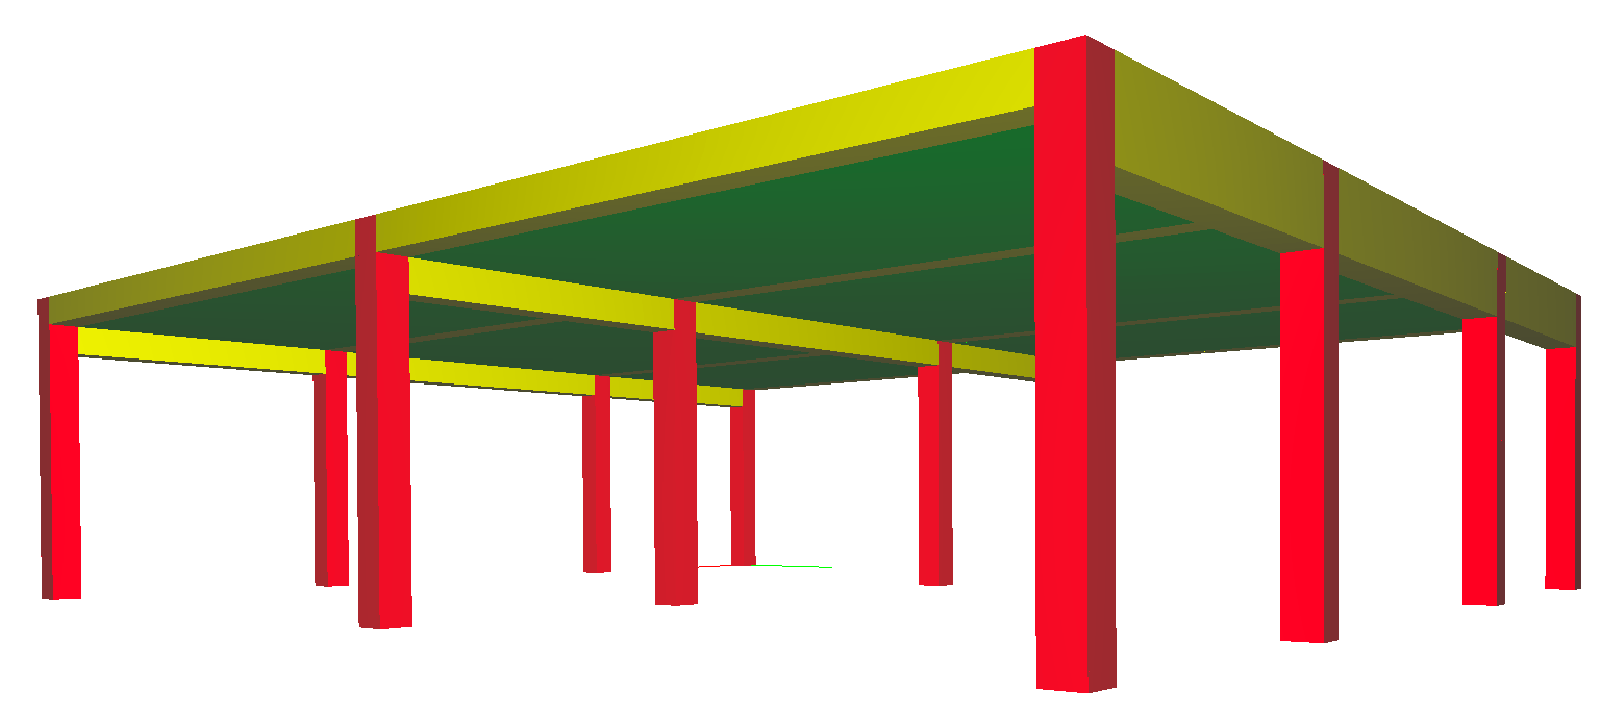
\includegraphics[width=\linewidth]{chapter-05/figs/frame1} 
   \caption{\sf frame = STRUCT(pillars, trusses, trusses1, floorslab);}.}
   \label{fig:example}
\end{figure}
\subsection*{Assembly combinator {\sf STRUCT}}\label{sect:5-1-1}

We have already come across the |STRUCT| function, one of more important |Plasm| operators. In particular, we already know that |STRUCT| is used to assembly geometric objects into a single object. In Julia |Plasm| both the input and the output objects are of recursive |Hpc| type.

In geometric modeling of complex assemblies the geometric and graphics
programmer makes wide use of the \emph{hierarchical scene
graphs}~\cite{Wernecke:94:TIM,Sowizral:2000:J3DAPI} or hierarchical
structures~\cite{Gaskins92}, where sub-assemblies are defined in \emph{local}
coordinates, and are transformed into the coordinate frame of the
output assembly by explicitly using proper coordinate
transformations.  

It is worth noting that such “modeling transformations" --- as they are called in graphical systems --- are left entirely to programmer's responsibility.  


\begin{figure}[htbp] %  figure placement: here, top, bottom, or page
   \sidecaption[t]
   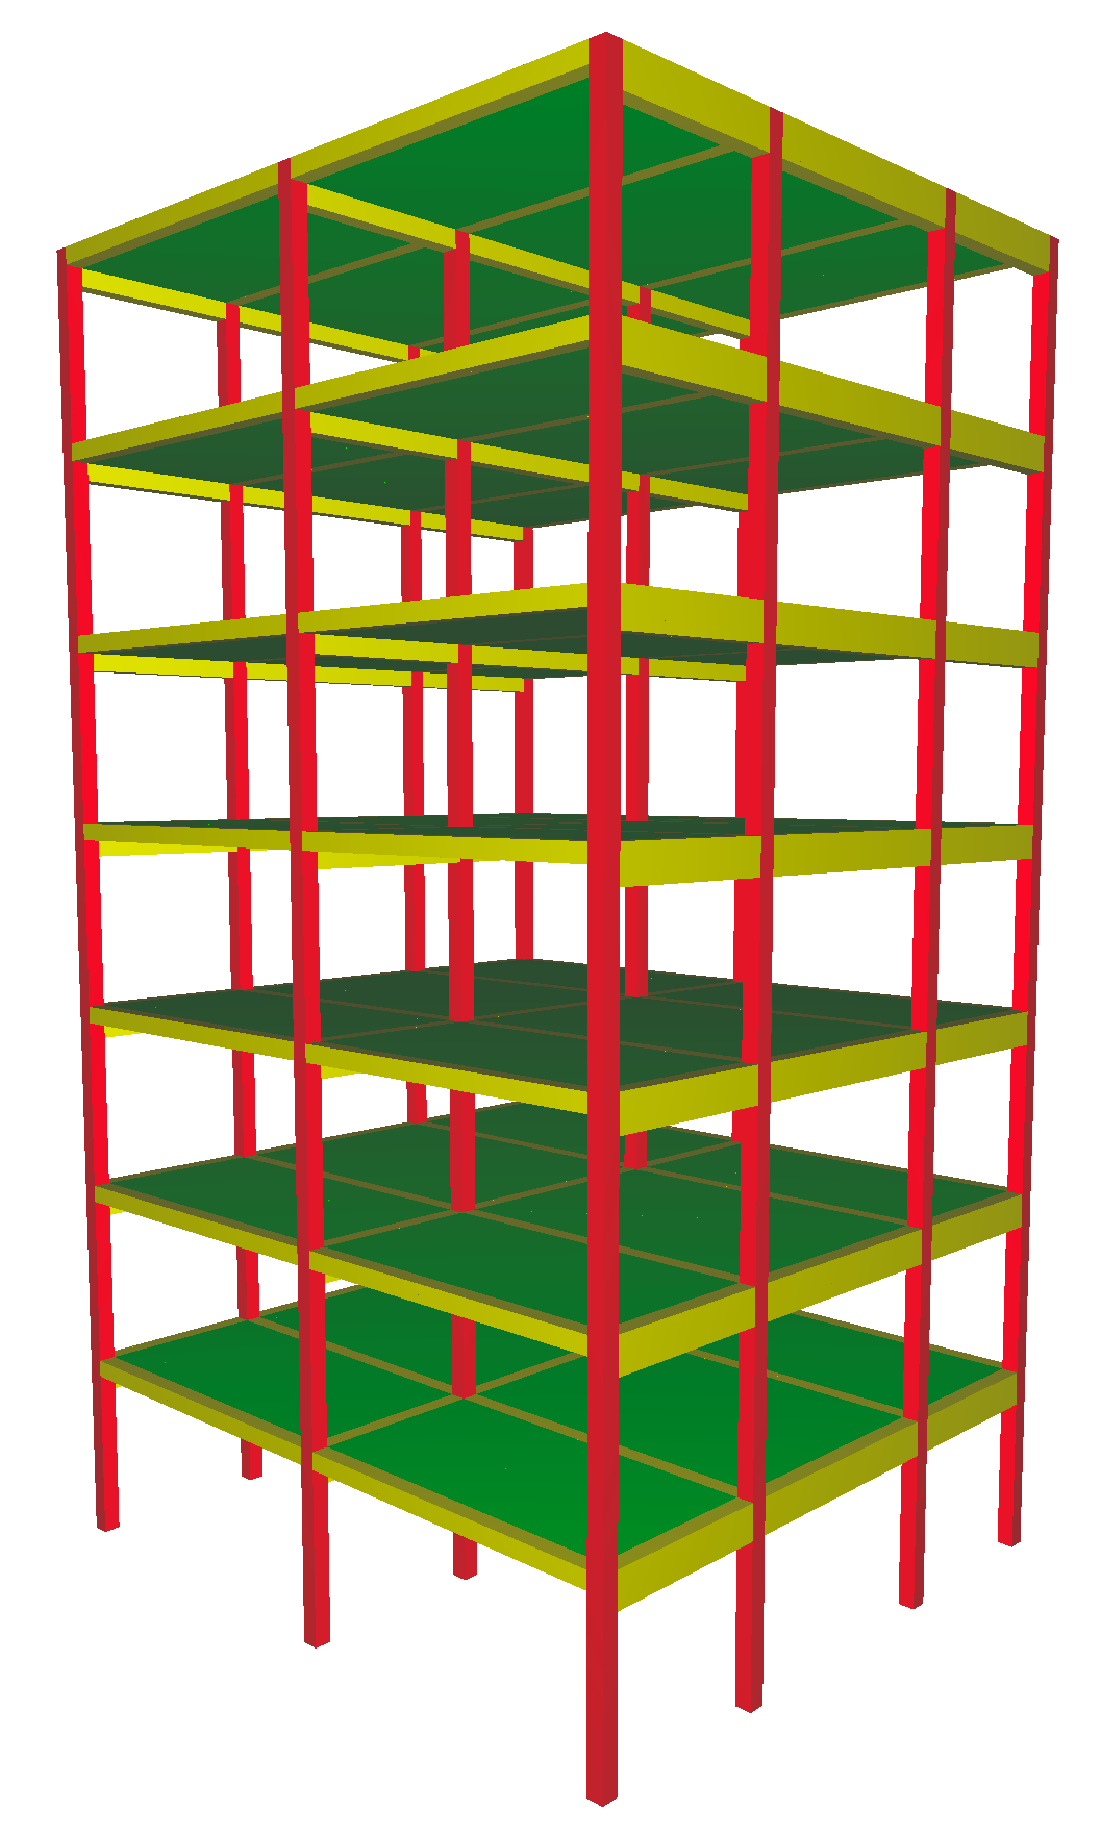
\includegraphics[width=0.6\linewidth]{chapter-05/figs/skeleton1} 
   \caption{\sf skeleton = STRUCT(NN(7)([frame, T(3)(3.3)])));}.}
   \label{fig:5:1:skeleton}
\end{figure}

\begin{coding}[Building skeleton]\label{5:1:skeleton}
We assemble here a building skeleton model, by creating a |STRUCT| assembly generated by |n=7| instances of the Julia |Vector| made by the |Hpc| value |frame| and by the |MatrixNd| value |T(3)(3.3)| producing a translation in $z$ direction.
\begin{lstlisting}[language=JuliaLocal, style=julia, mathescape=true]
skeleton = STRUCT(NN(7)([frame, T(3)(3.3)]));
VIEW(skeleton, Dict("background_color"=>WHITE)
\end{lstlisting}
\end{coding}

Here the |STRUCT| semantics is very clear: the evaluated subexpression |NN(7)([frame, T(3)(3.3)])| is an array of type |Vector{Union{Hpc, MatrixNd}}| and contain 14 item with alternating types.  When |STRUCT| is evaluted on this vector, an |Hpc| node is generated, whose |MatrixNd| field contains a $4\times 4$ identity matrix, and the |childs| vector contains the reference to the first item of 


\subsection*{Alignment aggregators {\sf TOP, BOTTOM, LEFT, RIGTH}}\label{sect:5-1-1}


In the present section we discuss some simplified assembly operators, where the
coordinate transformations are computed automatically by the language.

|Plasm| has some predefined binary functions used to locate two complexes with respect each other.  In particular,
the second argument of such functions will be positioned either
|TOP| the first one, or |ABOVE|, or |LEFT|, or
|RIGHT|, or |UP|, or |DOWN|, respectively,
according to the alignment semantics given below.

Such relative positioning allows
for an easy construction of complex assemblies, without taking into account the local coordinate frames where the
sub-assemblies are defined.  In this way we avoid applying affine transformations as it is
conversely needed in hierarchical scene graphs.

\begin{coding}[alternate method for vertical aggregation]\
\begin{lstlisting}[language=JuliaLocal, style=julia, mathescape=true]
multifloor(model,n) = STRUCT(INSR(TOP)(N(n+1)(model))) #=
multifloor (generic function with 1 method)		  	   =#
VIEW(multifloor(frame,7))
\end{lstlisting}
The object generated here is equal to the |skeleton| model of Figure \ref{fig:5:1:skeleton}. 
\end{coding}

|TOP| is a binary function of two |Hpc| models that creates their vertical aggregation.
Any binary function is transformed in $n$-ary by the second order operator |INSR| (for \emph{insert right}). |INSR| is applied first to the operator argument to make $n$-ary, then to the list of objects the operator apply to.

|N(n)(value::Any)| is a |Plasm| function called $\#$ in classic |PLaSM|, that returns a list of |n| instances of |value|. 

\begin{definition}[Primitive {\sf ALIGN} function.]
Every pair of polyhedral complexes may be aligned along any given subset of coordinates by using the primitive binary function |ALIGN|. Such a second-order operator must be applied to a sequence of triples which define a specialized behavior for each affected coordinate.
\end{definition}

Each alignment directive along a coordinate must belong to the set
\[
[1,n] \times \{ |MIN,MED,MAX,K($\alpha$)|\} 
\times \{ |MIN,MED,MAX,K($\alpha$})|\}
\]
where |$\alpha$::Number|. The resulting specialized operator is then applied to a pair of |Hpc| values, and returns a single |Hpc|. 
\begin{lstlisting}[language=JuliaLocal, style=julia, mathescape=true]
TOP = ALIGN([[3, MAX, MIN], [1, MED, MED], [2, MED, MED]])
BOTTOM = ALIGN([[3, MIN, MAX], [1, MED, MED], [2, MED, MED]])
LEFT = ALIGN([[1, MIN, MAX], [3, MIN, MIN]])
RIGHT = ALIGN([[1, MAX, MIN], [3, MIN, MIN]])
UP = ALIGN([[2, MAX, MIN], [3, MIN, MIN]])
DOWN = ALIGN([[2, MIN, MAX], [3, MIN, MIN]])
# 294 (generic function with 1 method)
\end{lstlisting}


\begin{figure}[htbp] %  figure placement: here, top, bottom, or page
   \sidecaption[t]
   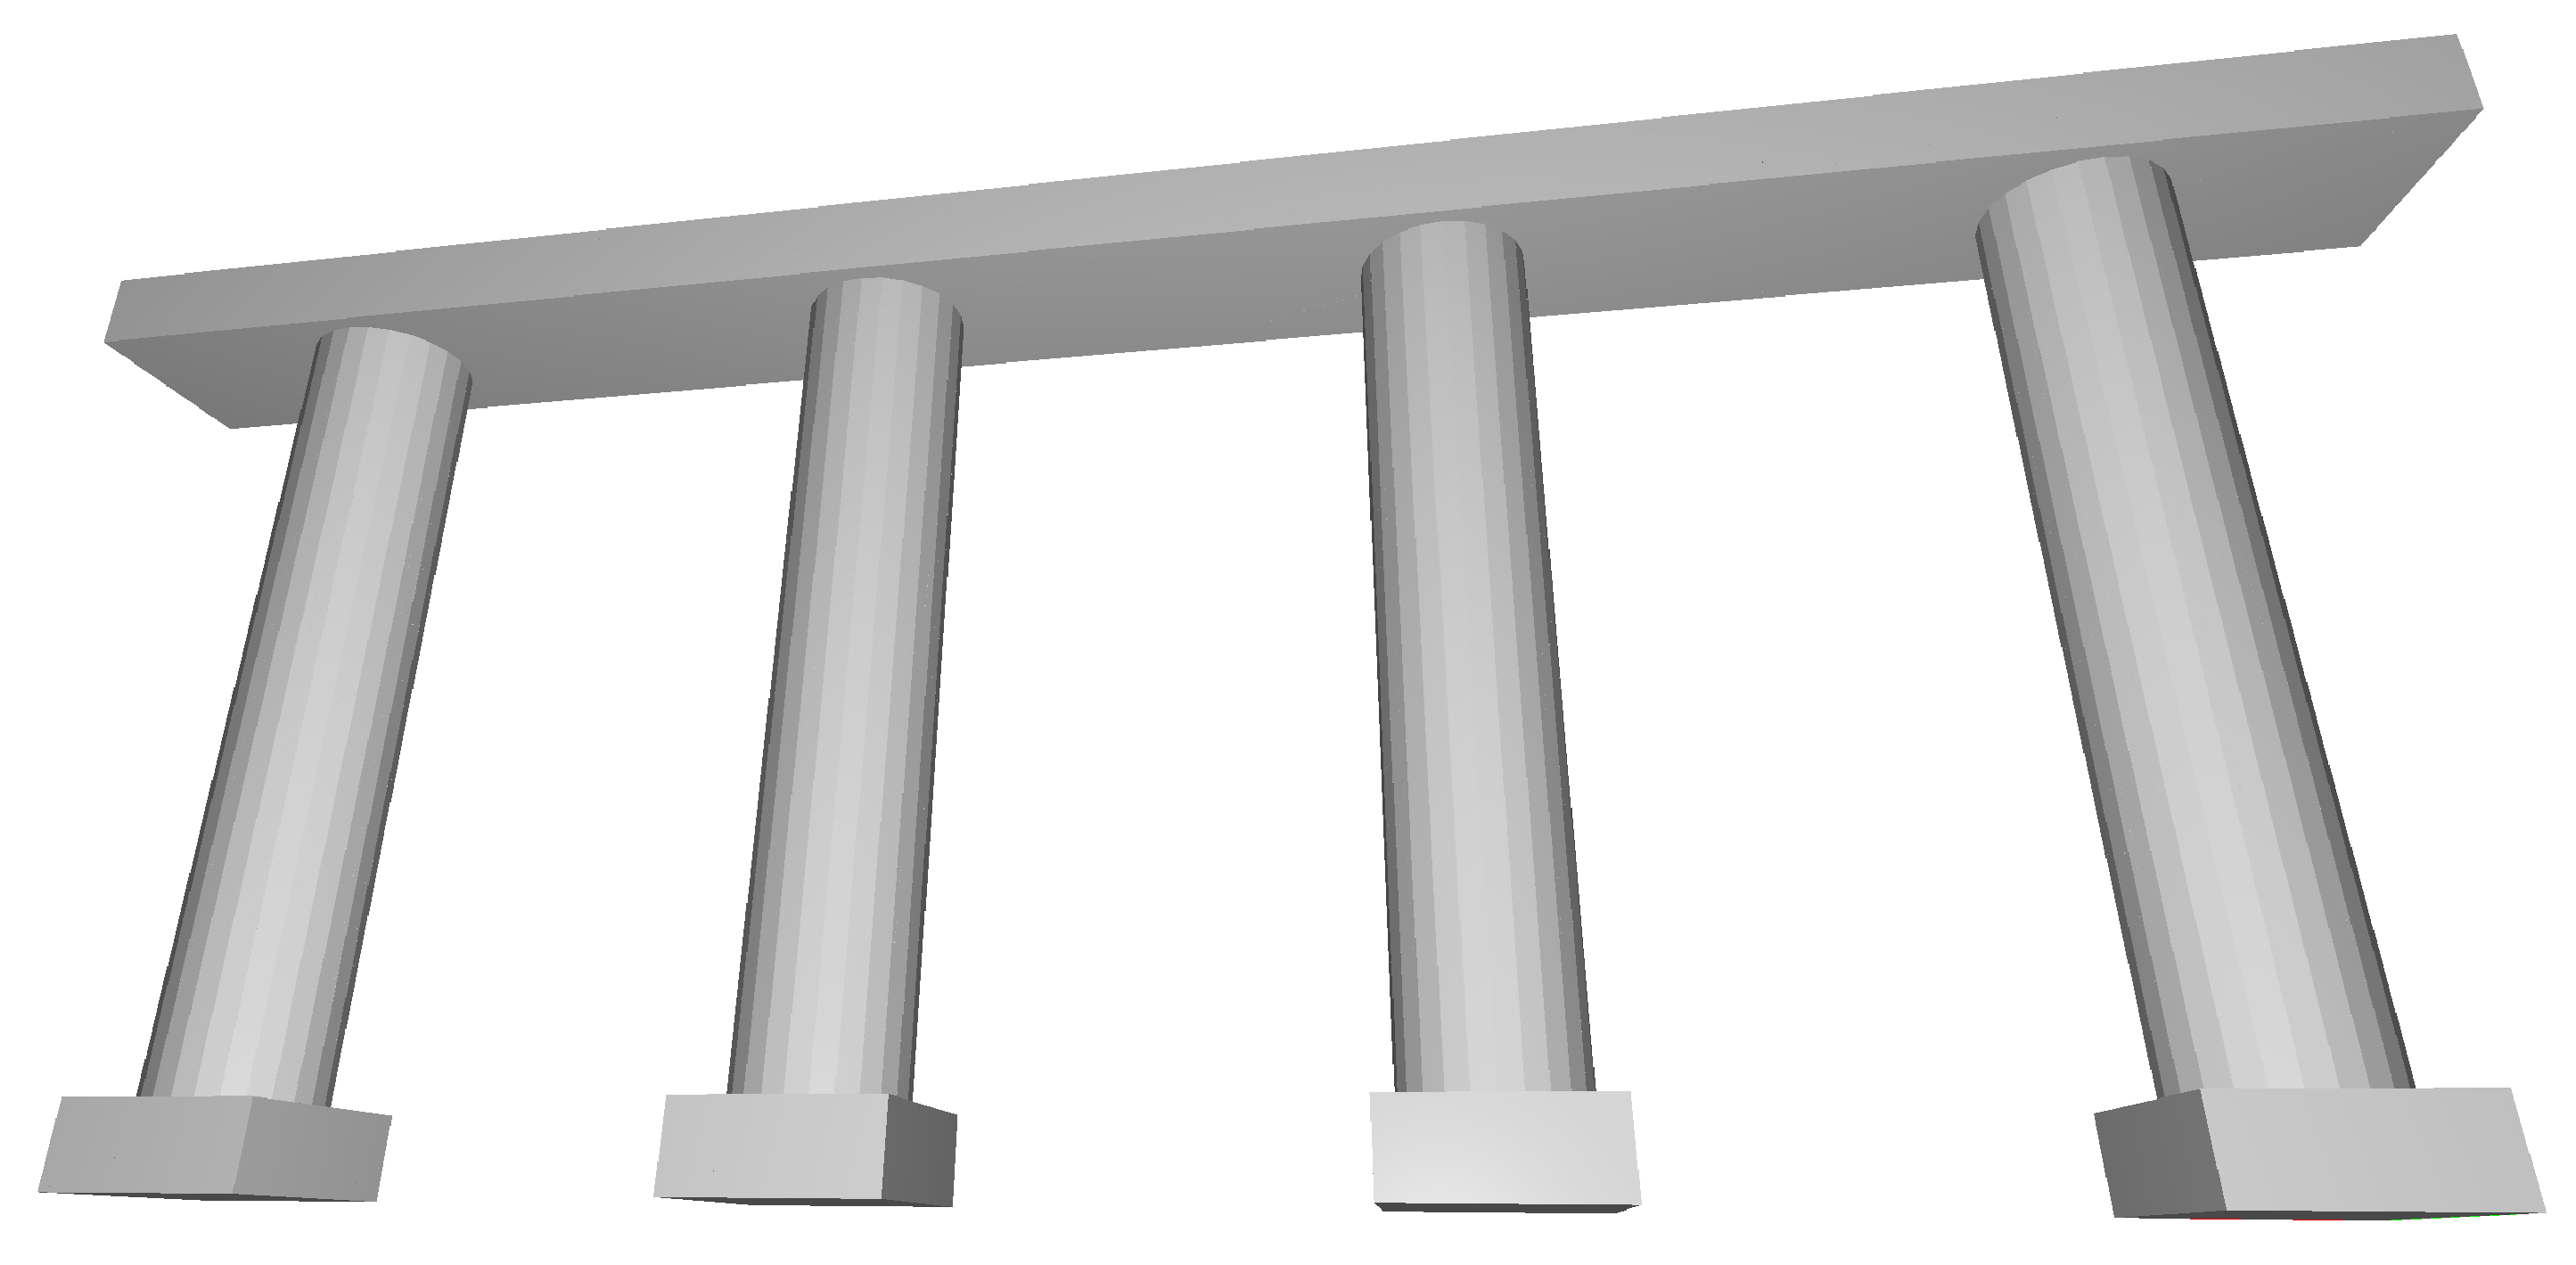
\includegraphics[width=\linewidth]{chapter-05/figs/fourcolumns} 
   \caption{\sf skeleton = STRUCT(NN(7)([frame, T(3)(3.3)])));}.}
   \label{fig:5:1:skeleton}
\end{figure}

\begin{coding}\
\begin{lstlisting}[language=JuliaLocal, style=julia, mathescape=true]
function Column(r::Float64,h::Float64)
	basis = CUBOID([ 2r*1.2, 2r*1.2, h/12 ]) 
	trunk = CYLINDER([ r, h/1.2 ])(24)
	capital = deepcopy(basis)
	beam = S(1)(3)(capital) 
	return INSR(TOP)([basis,trunk,capital,beam])
end
\end{lstlisting}

\begin{lstlisting}[language=JuliaLocal, style=julia, mathescape=true]
function ColRow(N::Int64)
	col = Column(1.0, 12.0)
	objs = [col for k in 1:N+1]
	return INSR(RIGHT)(objs)
end

VIEW(ColRow(4), Dict("background_color"=>WHITE)
\end{lstlisting}
\end{coding}


\section{ Plasm topological operators}\label{sect:5-2}


\section{ Linear and affine operators}\label{sect:5-3}


\section{ Manifold mapping}\label{sect:5-4}


\section{ Curve, surface, and solid methods}\label{sect:5-5}


